%%%%%%%%%%%%%%%%%%%%%%%%%%%%%%%%%%%%%%%%%%%%%%%%%%%%%%%%%%%%%%%%%%%%%%%%%%%%%
%%%
%%% File: thesis.tex, version 1.9, May 2016
%%%
%%% =============================================
%%% This file contains a template that can be used with the package
%%% cs.sty and LaTeX2e to produce a thesis that meets the requirements
%%% of the Computer Science Department from the Technical University of Cluj-Napoca
%%%%%%%%%%%%%%%%%%%%%%%%%%%%%%%%%%%%%%%%%%%%%%%%%%%%%%%%%%%%%%%%%%%%%%%%%%%%%

\documentclass[12pt,a4paper,twoside]{report}         
\usepackage{cs}              
\usepackage{times}
\usepackage{graphicx}
\usepackage{latexsym}
\usepackage{amsmath,amsbsy}
\usepackage{amssymb}
\usepackage[matrix,arrow]{xy}
\usepackage[T1]{fontenc}
\usepackage{ae,aecompl}
\usepackage{romanian} %definitii pentru diacritice; 
\usepackage{amstext}
\usepackage{graphics}
\usepackage[T1]{fontenc}
\usepackage{ae,aecompl}
%\usepackage{algorithm}
%\usepackage{algorithmic}
\usepackage{color}
\usepackage{color}
\usepackage{listings}
\usepackage{verbatim}
\usepackage{subcaption}

%\usepackage{algorithm2e}


% \mastersthesis
\diplomathesis
% \leftchapter
\centerchapter
% \rightchapter
\singlespace
% \oneandhalfspace
% \doublespace

\renewcommand{\thesisauthor}{Nicoleta COROCEA}    %% Your name.
\renewcommand{\thesismonth}{Iunie}     %% Your month of graduation.
\renewcommand{\thesisyear}{2019}      %% Your year of graduation.
\renewcommand{\thesistitle}{EXPLAINABLE MACHINE LEARNING USING ONTOLOGIES } % Title
\renewcommand{\thesissupervisor}{Assoc.Prof.Dr.Eng. Adrian GROZA}
\newcommand{\department}{FACULTATEA DE AUTOMATIC'A 'SI CALCULATOARE\\
DEPARTAMENTUL CALCULATOARE}
\newcommand{\thesis}{LUCRARE DE LICEN'T'A}
\newcommand{\uline}[1]{\rule[0pt]{#1}{0.4pt}}
%\renewcommand{\thesisdedication}{P'arin'tilor mei}
\newcommand{\utcnlogo}{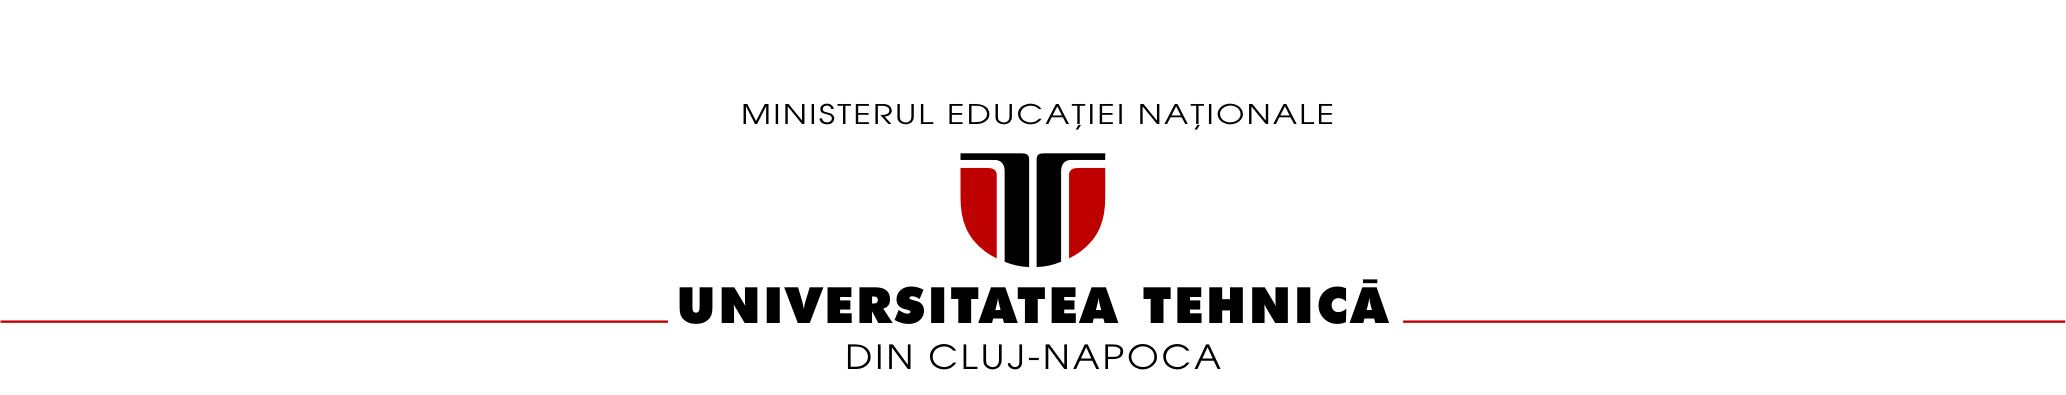
\includegraphics[width=15cm]{img/utcn.jpg}}
\newtheorem{example}{Exemplu}
\begin{document}

%\frontmatter
%\pagestyle{headings}

\newenvironment{definition}[1][Defini'tie.]{\begin{trivlist}
\item[\hskip \labelsep {\bfseries #1}]}{\end{trivlist}}



%\thesistitle                    %% Generate the title page.
%\authordeclarationpage                %% Generate the declaration page.


\begin{center}
%\includegraphics[width=15cm]{img/tucn.jpg}  
\utcnlogo

{\bf \department}

\vspace{4cm}

{\bf \thesistitle} %LICENSE THESIS TITLE}

\vspace{1.5cm}

\thesis

\vspace{6cm}

Absolvent: {\bf \thesisauthor} 

Conduc'ator 'stiin'tific: {\bf \thesissupervisor}

\vspace{3cm}
{\bf \thesisyear}
\end{center}

\thispagestyle{empty}
\newpage

\begin{center}
\utcnlogo

{\bf \department}
\end{center}
\vspace{0.5cm}

%\begin{small}
\begin{tabular}{p{7cm}p{8cm}}
 %\hspace{-1cm}& VIZAT,\\
 \hspace{-1cm}DECAN, & DIRECTOR DEPARTAMENT,\\
\hspace{-1cm}{\bf Prof. dr. ing. Liviu MICLEA} & {\bf Prof. dr. ing. Rodica POTOLEA}\\  
\end{tabular}
 
\vspace{2cm}

\begin{center}
Absolvent: {\bf \thesisauthor}

\vspace{1cm}

{\bf \thesistitle}
\end{center}

\vspace{1cm}

\begin{enumerate}
 \item {\bf Enun'tul temei:} {\it Scurt'a descriere a temei lucr'arii de licen't'a 'si datele ini'tiale}
\item {\bf Con'tinutul lucr'arii:} {\it (enumerarea p'ar'tilor componente) Exemplu: Pagina de prezentare, aprecierile coordonatorului de lucrare, titlul capitolului 1, titlul capitolului 2, titlul capitolului n, bibliografie, anexe.}
\item {\bf Locul document'arii:} {\it Exemplu}: Universitatea Tehnic'a din Cluj-Napoca, Departamentul Calculatoare
\item {\bf Consultan'ti:}
\item {\bf Data emiterii temei:} 1 Noiembrie 2018
\item {\bf Data pred'arii:} 8 iulie 2019 {\it (se va completa data pred'arii)}
  \end{enumerate}
\vspace{1.2cm}

\hspace{6cm} Absolvent: \uline{6cm} 

\vspace{0.5cm}
\hspace{6cm} Coordonator 'stiin'tific: \uline{5cm} 
%\end{small}

\thispagestyle{empty}

\newpage

\begin{center}
\utcnlogo

{\bf \department}
\end{center}

\vspace{0.5cm}

\begin{center}
{\bf
Declara'tie pe proprie r'aspundere privind\\ 
autenticitatea lucr'arii de licen't'a}
\end{center}
\vspace{1cm}



Subsemnatul(a) \\
\uline{14.8cm}, 
legitimat('a) cu \uline{4cm} seria \uline{3cm} nr. \uline{4cm}\\
CNP \uline{9cm}, autorul lucr'arii \uline{2.8cm}\\
\uline{16cm}\\
\uline{16cm}\\
elaborat'a 'in vederea sus'tinerii examenului de finalizare a studiilor de licen't'a la Facultatea de Automatic'a 'si Calculatoare, Specializarea \uline{7cm} din cadrul Universit'a'tii Tehnice din Cluj-Napoca, sesiunea \uline{4cm} a anului universitar \uline{3cm}, declar pe proprie r'aspundere, c'a aceast'a lucrare este rezultatul propriei activit'a'ti intelectuale, pe baza cercet'arilor mele 'si pe baza informa'tiilor ob'tinute din surse care au fost citate, 'in textul lucr'arii 'si 'in bibliografie.

Declar, c'a aceast'a lucrare nu con'tine por'tiuni plagiate, iar sursele bibliografice au fost folosite cu respectarea legisla'tiei rom\ia ne 'si a conven'tiilor interna'tionale privind drepturile de autor.

Declar, de asemenea, c'a aceast'a lucrare nu a mai fost prezentat'a 'in fa'ta unei alte comisii de examen de licen't'a.

'In cazul constat'arii ulterioare a unor declara'tii false, voi suporta sanc'tiunile administrative, respectiv, \emph{anularea examenului de licen't'a}.

\vspace{1.5cm}

Data \hspace{8cm} Nume, Prenume

\vspace{0.5cm}

\uline{3cm} \hspace{5cm} \uline{5cm}

\vspace{1cm}
\hspace{9.4cm}Semn'atura

\thispagestyle{empty}

\newpage

%\clearpage 
%\newpage

%\begin{comment}
{\color{red}{\bf De citit 'inainte} (aceast'a pagin'a se va elimina din versiunea final'a)}:
\begin{enumerate}
 \item Cele trei pagini anterioare (foaie de cap'at, foaie sumar, declara'tie) se vor lista pe foi separate (nu fa't'a-verso), fiind incluse 'in lucrarea listat'a. 
 Foaia de sumar (a doua) necesit'a semn'atura absolventului, respectiv a coordonatorului.
 Pe declara'tie se trece data c\ia nd se pred'a lucrarea la secretarii de comisie.
 \item Pe foaia de cap'at, se va trece corect titulatura cadrului didactic 'indrum'ator, 'in englez'a (consulta'ti pagina de unde a'ti desc'arcat acest document pentru lista cadrelor didactice cu titulaturile lor).
 \item Documentul curent {\bf nu} a fost creat 'in MS Office. E posibil sa fie mici diferen'te de formatare. 
\item Cuprinsul 'incepe pe pagina nou'a, impar'a (dac'a se face listare fa't'a-verso), prima pagin'a din capitolul Introducere tot a'sa, fiind numerotat'a cu 1. % Pentru actualizarea cuprinsului, click dreapta pe cuprins (zona cuprinsului va apare cu gri), Update field-$>$Update entire table.
\item Vizualiza'ti (recomandabil 'si 'in timpul edit'arii) acest document % după ce activaţi vizualizarea simbolurilor ascunse de formatare (apăsaţi simbolul  din Home/Paragraph).
\item Fiecare capitol 'incepe pe pagin'a nou'a. % datorită simbolului ascuns Section Break (Next Page) care este deja introdus la capitolul precedent. Dacă ştergeţi din greşeală simbolul, se reintroduce (Page Layout -> Breaks).
\item Folosi'ti stilurile predefinite (Headings, Figure, Table, Normal, etc.)
\item Marginile la pagini nu se modific'a.
\item Respecta'ti restul instruc'tiunilor din fiecare capitol.
\end{enumerate}
\thispagestyle{empty} 
%\end{comment}

\pagenumbering{roman}
\setcounter{page}{1}

\newpage

\tableofcontents

\newpage

%\listoftables
%\listoffigures

\pagenumbering{arabic}
\setcounter{page}{1}

%%%%%%%%%%%%%%%%%%%%%%%%%%%%%%%%%%%%%%%%%%%%%%%%%%%%%%%%%%%%%%%%%%%%%%%
\chapter{Introducere - Contextul proiectului}
\pagestyle{headings}
\section{Descrierea problemei}
\section{Conturarea solu'tiei}

%%%%%%%%%%%%%%%%%%%%%%%%%%%%%%%%%%%%%%%%%%%%%%%%%%%%%%%%%%%%%%%%%%%%%%%%%
\chapter{Obiectivele Proiectului}


\section{Pozi'tionarea sistemului}
\section{Descrierea obiectivelor}
\section{Cerin'tele sistemului}
\subsection{Cerin'te fun'tionale}
\subsection{Cerin'te nonfunc'tionale}

%%%%%%%%%%%%%%%%%%%%%%%%%%%%%%%%%%%%%%%%%%%%%%%%%%%%%%%%%%%%%%%%%%%%%%%%
\chapter{Studiu Bibliografic}
\textcolor{green}{-translatare limbaj natural
-limbaje de interogare
- XAI}


\section{Titlu}
\section{Alt titlu}

%%%%%%%%%%%%%%%%%%%%%%%%%%%%%%%%%%%%%%%%%%%%%%%%%%%%%%%%%%%%%%%%%%%%%%
\chapter{Analiz'a 'si Fundamentare Teoretic'a}
\label{ch:analysis}
\subsection{Ontologie}
\subsection{Quepy}
-parsare
- e framework
- creeaza un virtual env la instalare
- flexibilitatea intrebarilor este data manual, nu prin wordnet
\subsection{Aplica'tie Web Spring Boot}
\subsection{extragerea raspunsului}
\textcolor{green}{rdflib\&pellet - unele query-uri mergeau cu rdflib si nu mergeau cu quepy; diferenta intre cele doua + altele:hermit, racer}
\subsection{Interfa'ta utilizator}
\subsection{limbaje de interogare- sparql etc}
\subsection{Analiza arhitecturii}


%%%%%%%%%%%%%%%%%%%%%%%%%%%%%%%%%%%%%%%%%%%%%%%%%%%%%%%%%%%%%%%%%%%%%%%%
\chapter{Proiectare de Detaliu 'si Implementare}

\section{Arhitectura sistemului}

'In cadrul acestei sec'tiuni se prezint'a o scurt'a descriere a aplica'tiei, iar 'in sec'tiunile urm'atoare vor fi prezentate pe larg fiecare dintre componente. Agentul explicativ pune la dispozi'tie o interfa'ta pentru utilizator 'in care acesta poate introduce 'intrebari, respectiv poate afla rezultatul acestora 'si termeni cheie ai ontologiei. Serverul asigur'a translatarea 'in limbaj de interogare SPARQL a 'intrebarii ini'tiale, rularea interog'arii prin metoda aleas'a de client 'si afi'sarea r'aspunsurilor 'in zona destinata acestuia.

Arhitectura agentului explicativ pe domeniul machine-learning este structurat'a pe niveluri, 'in care fiecare modul este independent si constituie un nivel. Acest lucru permite ca unele func'tionalit'a'ti s'a fie solu'tionate printr-o aplica'tie Java, iar altele cu ajutorul scripturilor Python. Figura ~\ref{fig:arch} ilustreaz'a arhitectura general'a a sistemului 'si maniera 'in care cele patru module comunic'a 'intre ele. 'In cadrul acestor componente, modulul serverului pentru inferen't'a joac'a un rol major, dac'a nu principal, toate apelurile provenite de la interfa'ta utilizator fiind procesate de acesta. Func'tionarea corect'a a serverului este esen'tial'a 'in aceast'a aplica'tie, dar 'si translatorul Quepy 'si ontologia asigur'a comportamentul adecvat al sistemului.

Interac'tiunea utilizatorului cu interfa'ta const'a 'in introducerea unei intreb'ari 'in limbaj natural 'si ac'tionarea comenzii pentru transformarea in limbajul de interogare SPARQL. Apelul va fi tratat de serviciul de inferen't'a {\it Reasoning Service}, prezentat 'in Fig. ~\ref{fig:arch}, care va realiza transformarea cu ajutorul translatorului Quepy, denumit 'in figura citata {\it Quepy translator}. Interogarea SPARQL va fi afi'sat'a 'si clientul are posibilitatea de a o modifica sau de a o executa fie folosind libraria Pellet, fie cu script-ul care utilizeaz'a RDFLib. R'aspunsul va fi prezentat 'in aria destinat'a. Utilizatorul mai are la dispozi'tie 'si o pagin'a 'in care poate solicita detaliile ontologiei: listarea claselor, a indivizilor 'si a propriet'a'tilor care le leag'a.


\begin{figure}[h!]
    \centering
    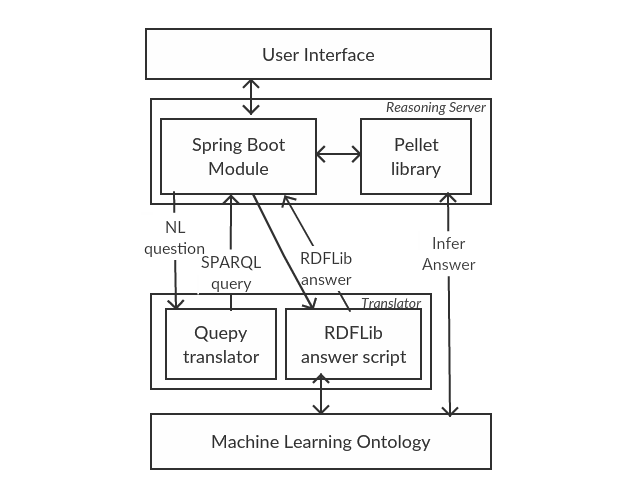
\includegraphics[width = 0.75\linewidth]{img/arhitectura-generala-black.png}
        \caption{Arhitectura sistemului}
    \label{fig:arch}
\end{figure}

Interfa'ta utilizator este construit'a simplu, 'in stil minimalist, astfel 'incat clientul s'a nu se piard'a 'in detalii. Este alc'atuit'a din dou'a pagini cu ajutorul c'arora utilizatorul poate chestiona datele 'in limbaj natural cu ajutorul librariei Pellet sau RDFLib sau poate ob'tine detalii despre ontologie. 

Serverul pentru inferen't'a, 'in imaginea mai sus men'tionat'a {\it Reasoning Service}, este consituit din libr'aria Pellet 'in care am integrat un modul Spring Boot pentru a pune la dispozi'tie sub form'a de endpoint-uri func'tionalit'a'tile necesare. Ca arhitectur'a, este format dintr-un nivel de control, un nivel de  servicii pentru ob'tinerea informa'tiilor de la libr'aria Pellet si de la modulul Python care utilizeaz'a RDFLib, 'si un nivel inferior pe care se afl'a libr'aria pentru inferen't'a.

Pe cel de-al treilea nivel al arhitecturii generale este pozi'tionat modulul Python denumit {\it Translator}. Acesta are doua func'tionalit'a'ti, o func'tionalitate pentru translatarea 'intreb'arilor din limbaj natural 'in SPARQL 'si una pentru interogarea ontologiei folosind libr'aria RDFLib. Translatorul Quepy este generat automat cu ajutorul framework-ului Quepy 'si con'tine clasele standard pentru parsare, pentru 'in'telegerea limbajului specific al domeniului 'si pentru ini'tializarea aplica'tiei. La acestea, se adaug'a un script pentru ob'tinerea unui r'aspuns cu ajutorul libr'ariei RDFLib.

Nivelul inferior const'a 'in ontologie, reprezent'and componenta care asigur'a persisten'ta datelor referitoare la machine learning. Indivizii acesteia sunt structura'ti 'in clase si subclase, depinz\ia nd unul de altul prin propriet'a'ti. O detaliere a arhitecturii ontologiei, c\ia t 'si a func'tionalita'tii 'si implement'arii fiec'arei componente mai sus amintite, va fi prezentat'a 'in cardul acestui capitol, 'in sec'tiunile care urmeaz'a. 

'In Figura ~\ref{fig:arch_det} se prezint'a modulele principale ale sistemului, 'impreuna cu modul detaliat de comunicare al acestora. Fluxul de informa'tii porne'ste de la utilizator 'si str'abate serverul pentru inferen't'a, {\it Reasoning Server}. 'In situa'tia 'in care s-a f'acut un apel pentru translatarea unei 'intreb'ari din limbaj natural 'in SPARQL sau pentru ob'tinerea r'aspunsului prin RDFLib, este utilizat 'si modulul {\it Translator}, 'in fun'tie de cerin'te. 

\begin{figure}
    \centering
    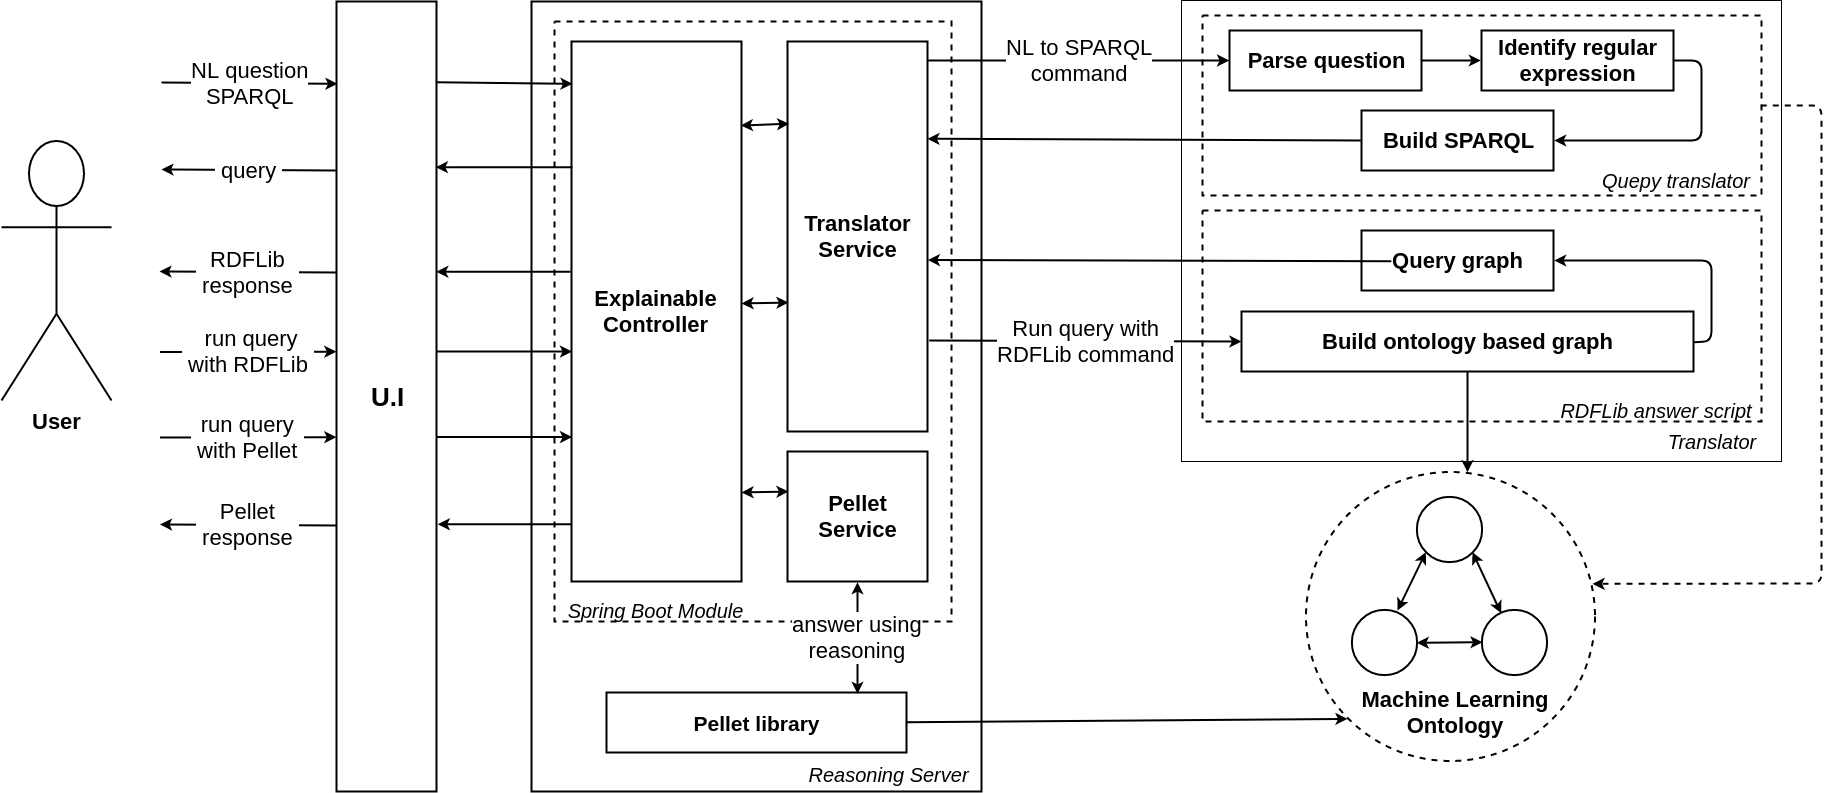
\includegraphics[width = 0.75\linewidth]{img/architecture_details.png}
        \caption{Elemente de comunicare 'in arhitectur'a}
    \label{fig:arch_det}
\end{figure}

Imaginea mai sus amintit'a pune 'in valoare trei situa'tii principale, care sunt folosite 'in mod global: translatarea unei 'intrebari 'in SPARQL cu ajutorul libr'ariei Quepy, interogarea r'aspunsului prin Pellet sau prin RDFLib. 'In toate aceste cazuri, se utilizeaz'a ontologia 'incarcat'a in memoria aplica'tiei sau se face uz de abstractizarea acesteia 'in cod, pentru modulul translatorului Quepy.

Primul pas al utilizatorului este de a insera 'intrebarea si de a activa apelul translat'arii acesteia. Serverul constituit din modulul Spring Boot va intercepta cerint'a 'in {\it Explainable Controller} 'si o va trece mai departe la serviciul dedicat, {\it Translator Service}. Acesta din urm'a execut'a comanda de rulare a modulului {\it Quepy translator}. Translatorul parseaz'a 'intrebarea, identific'a expresia regulat'a cu care se potrive'ste 'si contruie'ste interogarea SPARQL dintr-un graf generat de acest proces, apoi pune la dispozi'tie r'aspunsul pentru a fi preluat de {\it Reasoning Server}. Ca r'aspuns al apelului f'acut de utilizator, serverul va returna interogarea, iar aceasta va fi afi'sat'a 'in interfa'ta utilizator.

De'si primul pas poate fi omis 'si clientul poate s'a introduc'a manual interogarea pe care o dore'ste, rularea interog'arii aferente 'intreb'arii utilizatorului constituie al doilea pas logic 'in execu'tia cerin'tei. Utilizatorul activeaz'a comanda pentru rulare cu Pellet sau cu RDFLib din interfa'ta utilizator. 'In ambele cazuri, 'si atunci c'and dore'ste aflarea r'aspunsului prin inferen'ta sau prin extragere din graf, apelul va fi recep'tionat de controller. 

Dac'a ne afl'am 'in situa'tia 'in care se dore'ste aflarea r'aspunsului prin Pellet, controllerul  va 'inainta cererea la {\it Pellet Service}. Acesta o va solu'tiona cu ajutorul libr'ariei Pellet care de'tine modelul ontologiei 'in memorie 'si va extrage r'aspunsul prin reasoning. Astfel, 'si solu'tiile mai pu'tin evidente vor fi incluse 'in r'aspuns. R'aspusul este formatat de c'atre {\it Pellet Service} 'in format JSON pentru o lizibilitate crescut'a.

Solu'tionarea r'aspunsului prin graful RDFLib const'a in 'inaintarea apelului c'atre script-ul de ob'tinere a r'aspunsului bazat pe RDFLib, implementat 'in {\it Translator}. Pentru aflarea r'aspunsului, aceasta func'tie va citi ontologia sub form'a de graf RDF de la locatia precizat'a. Acest model RDF al ontologiei va fi interogat cu ajutorul query-ului transmis ca parametru 'si va returna un JSON cu rezultatele. Serviciul responsabil cu preluarea rezultatului este {\it Translator Service}. Acesta va returna controllerului rezultatul, care mai departe le va transmite interfe'tei utilizator, unde vor fi afi'sate.

Aplica'tia prezentat'a are o arhitectur'a structurat'a pe niveluri, oferind independe't'a 'intre module. Acest fapt aduce cu sine avantaje cum ar fi: func'tionarea aplica'tiei pe baza interogarilor directe 'in SPARQL 'in cazul 'in care modulul {\it Translator} nu func'tioneaz'a; 'inlocuirea ontologiei cu alta dintr-un domeniu diferit; asignarea atribu'tiilor clare 'si separate modulelor. 




\section{Modulul interfe'tei utilizator}
\textcolor{green}{- transparenta in pasii parcursi ; 
cum sustine xai}

\section{Modulul de raspuns bazat pe reasoner}

{\it Reasoning Server} reprezint'a punctul central al aplica'tiei, fiind modulul care rezolv'a cererile utilizatorilor. Acesta este un modul Spring Boot, integrat 'in libr'aria Pellet ce deleag'a componentele spre a 'indeplini sarcinile cerute de utilizator. 'In figura ~\ref{fig:uml_server} este prezentat'a o parte important'a a serverului, respectiv clasele implementate de mine 'impreuna cu cele din libr'aria Pellet de care depind.
\begin{figure}[h!]
    \centering
    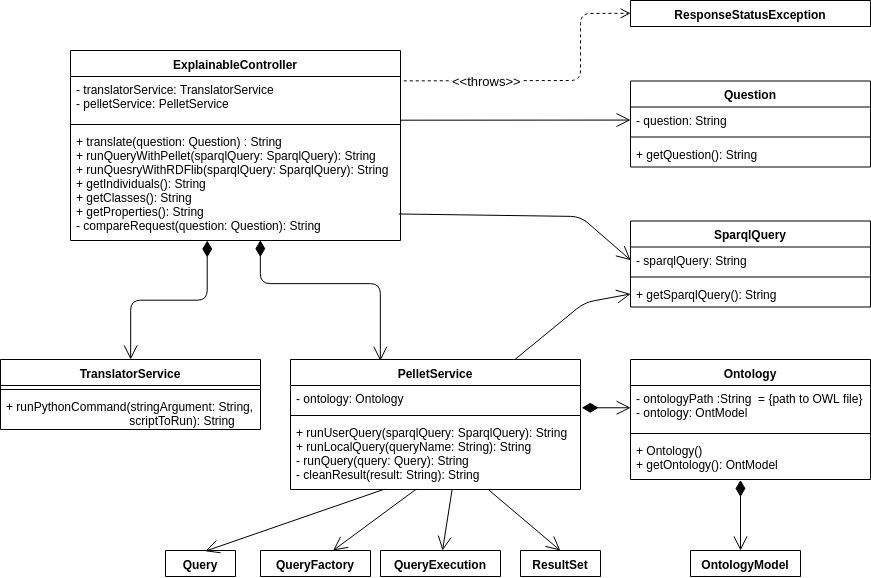
\includegraphics[width = 0.75\linewidth]{img/uml_server.png}
        \caption{Diagrama de clase a serverului {\it Reasoning Server}}
    \label{fig:uml_server}
\end{figure}

'In diagrama din figura ~\ref{fig:uml_server}, {\it ExplainableController} 'indepline'ste func'tia de controller al aplica'tiei. Este format din $translatorService$ 'si $pelletService$ a c'aror instan'te sunt aduse prin injectarea dependin'telor. Acestea au rolul de 'indeplinire a serviciilor, respectiv a logicii mai complexe pentru ob'tinerea r'aspunsurilor. $PelletService$ con'tine o instan't'a a ontologiei, $ontology$. Aceasta, la r\ia ndul ei este ob'tinut'a cu ajutorul fi'sierului OWL 'si a modelului pus la dispozi'tie de Pellet, $OntModel$. 'In plus fa't'a de $Ontology$, consider c'a clasele $Question$, $SparqlQuery$ sunt alte doua clase ce apar'tin modelului aplica'tiei, fiind utile 'in 'incapsularea datelor din request-uri.

$Query$ 'si $QueryFactory$ abstractizeaz'a o interogare 'in forma SPARQL care urmeaz'a a fi utilizat'a de Pellet pentru a ob'tine un r'aspuns de tipul $ResultSet$ prin intermediul $QueryExecution$. Acestea sunt clase care fac parte din libr'aria Pellet 'si nu le vom detalia.

Metoda $translate$ este apelat'a prin intermediul endpoint-ului {\it /translateQuery} 'si con'tinutul datelor transmise este un obiect din clasa $Question$, fiind o abstractizare a 'intreb'arii utilizatorului. Este utilizat'a pentru translatarea 'intreb'arii din limbaj natural 'in limbaj de interogare SPARQL.  Dac'a prin 'intrebare utiliztorul solicit'a compararea a doi algoritmi, se va utiliza metoda $compareRequest$ 'si se va returna o interogare SPARQL construit'a local. Altfel, aceasta apeleaz'a metoda $runPythonCommand$ din $TranslatorService$ 'si returneaz'a rezultatul dat de Quepy c'atre interfa'ta utilizator. Asem'an'ator, $runQueryWithRDFLib$ din controller este atins'a prin intermediul rutei {\it /runQueryWithRDFLib} 'si apeleaz'a aceea'si metod'a pentru rulare a comenzii din $TranslatorService$, preciz\ia nd de data aceasta script-ul de ob'tinere a r'aspunsului cu RDFLib.

Metoda $runQueryWithPellet$ este folosit'a pentru ob'tinerea r'aspunsului la interogarea SPARQL print intermediul Pellet. Utilizeaz'a path-ul {\it /runQueryWithPellet} 'si va apela $runUserQuery$ din $PelletService$. 'In $runUserQuery$ se stabile'ste interogarea SPARQL a utilizatorului 'si se apeleaz'a $runUserQuery$. Prin $runQuery$, r'aspunsul este ob'tinut de la Pellet 'in format JSON utiliz'and clasele $QueryExecution$ 'si $ResultSet$, urm'and ca apoi acesta s'a fie cur'a'tat de prefixuri prin intermediul metodei $cleanResult$.

Metodele $getClasses$, $getIndividuals$ 'si $getProperties$ sunt accestate prin intermediul path-urilor $/classes$, $/individuals$ 'si respectiv $/properties$. Acestea au rolul de a ob'tine toate clasele ontolgiei, to'ti indivizii 'si toate propriet'a'tile. Utilizeaz'a metoda $runLocalQuery$ 'si interog'ari 'in limbaj SPARQL definite local. Pentru ob'tinerea r'aspunsului se folose'ste metoda $runQuery$, asem'an'ator cazului 'in care se utilizeaz'a interogarea utilizatorului.

Libr'aria Pellet reprezint'a suportul pentru modulul $Reasoning\ Server$ 'si realizeaz'a ob'tinerea r'aspunsului prin inferen'ta. Prin intermediul $ExplainableController$, utilizatorul are acces la translatarea din limbaj natural 'in limbaj de interogare SPARQL, c'at 'si la interogarea ontologiei prin Pellet sau prin RDFLib.



\section{Modulul de raspuns pe baza de graf}

Acest modul este destinat interog'arii ontologiei aflat'a 'in forma de graf RDF 'si folose'ste RDFLib pentru a pune 'in practic'a acest lucru. Utilizarea libr'ariei RDFLib este simpl'a, fiind necesar'a doar instalarea 'si importarea acesteia. Modulul 'in care am implementat interogarea ontologiei 'in format RDF este un script 'si vine 'in ajutor pentru momentele 'in care un query SPARQL are anumite particularit'a'ti semantice care nu sunt interpretate 'in acela'si mod de Pellet. 

\begin{figure}
\centering
\begin{lstlisting}[language=Python, basicstyle=\footnotesize,numbers=left, xleftmargin=.05\textwidth]
import json, re, sys
from rdflib import Graph

PREFIXES = ["http://www.semanticweb.org/machine-learning-ontology#",  
            "http://www.w3.org/2002/07/owl#"]


def to_json(query_response):
    list_result = []
    for row in query_response:
        dictionary_response = {}
        for i in range(len(row)):
            current_result = row[i]
            for prefix in PREFIXES:
                if prefix in row[i]:
                    current_result = re.sub(prefix, "", row[i])
            dictionary_response[row.labels.keys()[row.labels.values().index(i)]] \
                = current_result
            list_result.append(dictionary_response)

    json_result = json.dumps(list_result, sort_keys=False, indent=4)
    return json_result


query = sys.argv[1]
g = Graph()
g.parse(r'../ontologies/machine-learning-ontology.owl', format="xml")
query_response = g.query(query)
json_result = to_json(query_response)
print json_result

\end{lstlisting}
        \caption{Scriptul pentru interogare prin RDFLib}
      \label{fig:rdflib_script}
\end{figure}

'In figura ~\ref{fig:rdflib_script} primul pas 'in ob'tinerea unui r'aspuns la o interogare SPARQL este de a citi de la linia de comand'a interogarea SPARQL care a fost transmis'a, 'in cazul aplica'tiei noastre, de c'atre serviciul aferent din {\it Reanoning Service}. La liniile (26)-(25), se formeaz'a un graf 'si ontologia noastr'a este parsat'a si salvat'a sub forma de noduri de triple. 'In continuare, la linia (28), se afl'a r'aspunsul interog'arii SPARQL. R'aspunsul dat de RDFLib nu este compatibil cu formatul JSON 'si con'tine informa'tii despre prefixe care ar putea induce 'in eroare utilizatorul. Astfel c'a, am implementat func'tia $to\_json(query\_response)$, ilustrat'a 'in figura ~\ref{fig:rdflib_script} la liniile (8-22), pentru a transforma r'aspunsul in format JSON 'si a-l 'infrumuse'ta. 

'In final, raspunsul $json\_result$ va fi printat 'si preluat de c'atre server. Dup'a cum am mai amintit 'in acest capitol, r'aspunsul este trimis de c'atre server la interfa'a utilizator, unde va fi vizualizat de c'atre client.


\section{Modulul de translatare}
\subsection{Arhitectura 'si func'tionarea translatorului Quepy}


Modulul $Translator$ este construit 'in Python cu ajutorul framework-ului Quepy. Este destinat pars'arii 'si translat'arii 'intreb'arilor din limbaj natural 'in limbaj de interogare SPARQL. Modulul este generat automat de o comand'a quepy, iar 'in figura ~\ref{fig:quepy_files} se pot observa componentele acestuia. 
\begin{figure}
    \centering
    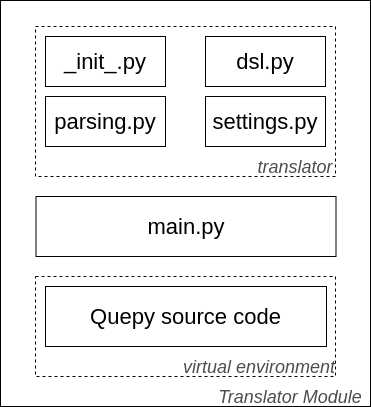
\includegraphics[width = 0.45\linewidth]{img/quepy_schema.png}
    \caption{Caption}
    \label{fig:quepy_files}
\end{figure}

Fi'sierul $\_init\_.py$ constituie punctul de plecare al aplica'tiei, fi'sierul de ini'tializare. 'In acesta se import'a fi'sierul $parsing.py$, iar la instalarea aplica'tiei va fi citit prin intermediul $\_init\_.py$. 

Unul dintre cele mai importante fi'siere ale acestui modul este $parsing.py$. Acesta con'tine toate regulile de parsare ale aplica'tiei. 'In acest fi'sier sunt declarate toate 'intreb'arile, sub forma de patternuri. 'In sec'tiiunea ~\ref{sec:parse} vom detalia acest fi'sier, 'impreuna cu procedeul de dezvoltare.

Fi'sierul $settings.py$ presupune locul 'in care se declara toate prefix-urile necesare unei interog'ari SPARQL, cum ar fi 'in cazul nostru prefixul pentru ontologia noastr'a 'si altele. Tot 'in acest loc, se decide limbajul de interogare, care 'in modulul $Translator$ este SPARQL.

Limbajul specific al domeniului este definit in $dsl.py$, fi'sier 'in care am adaugat toate clasele ontologiei noastre, 'impreuna cu propriet'a'tile acestora. Modul de detaliere al ontologiei, exemple de clase din acest fi'sier 'si o descriere mai larga a acestuia sunt 'in sec'tiunea ~\ref{sec:dsl}.

'In continuare voi prezenta algoritmul ~\ref{alg:quepy} care reprezint'a fluxul de procesare al unei 'intreb'ari 'in cadrul aplica'tiei Quepy pentru a fi transformat'a 'in limbaj de interogare SPARQL.

  

Inputul algoritmului este o 'intreare 'in limbaj natural, $q$. Primul pas const'a 'in extragerea tuturor regulilor definite 'in aplica'tie. Apoi, 'intrebarea utilizatorului este 'imp'ar'tit'a 'in tokeni, 'si i se atribuie etichete care identific'a ce parte a vorbirii este (substantiv, verb, prepozi'tie etc.), ob'tin\ia nd $W_q$. Rezultatul $q_{SPARQL}$ este 'ini'tializat. Pentru fiecare regul'a definit'a 'in mul'timea de reguli se verific'a dac'a se potrive'ste cu $W_q$. 'In cazul 'in care se potrive'ste, se ob'tine clasa 'in care a fost definit'a regula 'si 'in func'tie de metoda de interpretare, se adaug'a un noduri 'in graf care con'tin o tripl'a surs'a - proprietate - destina'tie. Se returnez'a interogarea SPARQL dup'a ce graful a fost interpretat. 'In cazul 'in care nu a fost indentificat'a o regul'a potrivit'a, se returneaz'a o interogare goal'a.

\subsection{'Incorporarea elementelor ontologiei 'in Quepy}
\label{sec:dsl}

Pentru a putea construi interog'ari potrivite pentru o ontologie, modulul Quepy trebui customizat pentru a cunoa'ste clasele 'si propriet'a'tile din ontologie, c\ia t 'si alte reguli care sunt necesare a fi integrate 'in interog'ari. 'In fi'sierul $dsl.py$ am definit clasele asem'an'ator exemplului de cod ~\ref{lst:learning_meth_op}: 
\begin{lstlisting}[basicstyle=\footnotesize, language = Python, label = lst:learning_meth_op, caption = Clasa LearningMethod]
   class IsLearningMethod(FixedType):
    fixedtype = "ml:LearningMethod"

    def __init__(self, operator):
        super(IsLearningMethod, self).__init__(operator)
        self.fixedtype = operator + "ml:LearningMethod"

\end{lstlisting}

Acesta este un exemplu 'in care am 'incadrat 'si 'imbun'at'a'tirile aduse libr'ariei, 'si anume suportul pentru o operatorii logici. Propriet'a'tile sunt definite asem'an'ator cu exemplul de cod ~\ref{lst:learning_meth_rel}:

\begin{lstlisting}[basicstyle=\footnotesize, language = Python, label = lst:learning_meth_rel, caption = Proprietatea has-learning-method]
class HasLearningMethodReversed(FixedRelation):
    relation = "ml:has-learning-method"
    reverse = True

class NotHasLearningMethod(MinusFixedRelation):
    relation = "ml:has-learning-method"
    reverse = False

class HasLearningMethod(FixedRelation):
    relation = "ml:has-learning-method"
    reverse = False

\end{lstlisting}

'In acest exemplu am 'incadrat rela'tia invers'a, rela'tia implementat'a de mine pentru a sus'tine operatorul $minus$ cu func'tia de $not$, 'si rela'tia simpl'a.


\subsection{Parsarea 'intreb'arilor}
\label{sec:parse}





\textcolor{green}{ cum arata fisierul parsing.py}

\textcolor{green}{exemplu de parsare: }
'In fisierul $parsing.py$ am definit toate regulile de parsare ale 'intreb'arilor, un num'ar total de 15 clase asociate ficare c\ia te unei 'intreb'ari. Acestea con'tin regulile de parsare, 'impreuna cu o metod'a $interpret$ care specific'a ordinea 'in care vor fi ad'augate elementele identificate 'in interogare.
Figura ~\ref{fig:r1} detaliaz'a regula pentru identificarea indivizilor clasei $Algorithm$. 'In aceast'a regul'a, $target$ func'tioneaz'a ca 'inlocuitor pentru conceptul c'aruia dorim s'a 'i afi'sam indivizii. Poate fi substantiv (NN), substantiv propriu (NNP) sau substantiv la plural (NNS). Variabila $optional\_opening$ este un 'inlocuitor pentru {\it"What are the"} sau {\it"Which are the"} 'si este op'tional'a, a'a cum este definit de comportamentul func'tiei $Question$. Prin $Lemma("be")$ 'in'telegem cuv\ia ntul de baz'a 'si inflexiunile sale, adic'a toate formele verbului $"to\ be"$.
Expresiile $regex1$ 'si $regex2$ sunt cuprinse 'in $regex$ 'si reprezint'a toate formele acceptate ale 'intreb'arii.

\begin{figure}[h]
\centering
\begin{lstlisting}[basicstyle=\footnotesize, numbers=left, xleftmargin=.05\textwidth]
target = Group (Pos("NN") | 
                Pos("NNP") | 
                Pos("NNS"), "target")
opt_opening = Question((Pos("WP") | 
                        Pos("WDT")) + 
                          Lemma("be") + 
                          Pos("DT"))
regex1 = optOpening + 
         Question(Lemma("individual") | 
                  Lemma("instance")) + 
                    Pos("IN") + target + 
                    Question(Pos("."))
regex2 = Question(Lemma("list") | 
                  Lemma("show") | 
                  Lemma("print")) + target +   
                  Question(Lemma("individual") |
                           Lemma("instance"))
regex = regex1 | regex2
  \end{lstlisting}
        \caption{Rule $R_1$ for listing individuals.}
      \label{fig:r1}
  \end{figure}
  
  \begin{example}[Applying $R_1$] 
  Fie 'intrebarea {\it What are the individuals of Algorithm?}
  Aceasta face match pe $regex1$ dup'a cum urmeaz'a:
  
   %\begin{table}[h]
%      \caption{regex and matching words}
 %     \centering
 %\vspace{0.3cm}
 \begin{center}
      \begin{tabular}{ll}
      regex part & word\\ \hline
      
  {\it Pos("WP")} & What\\
  {\it Lemma("be")} & are\\
  {\it Pos("DT")} & the\\
  {\it Lemma("individual")} & individuals\\
  {\it Pos("IN")} & of\\
  {\it target} & Algorithm\\
       \end{tabular}
       \end{center}
        \vspace{0.3cm}
   \end{example}
 

\subsection{'Imbun'at'a'tiri aduse libr'ariei Quepy}





% \subsubsection{Query Rules}

\textcolor{green}{pornind de la intrebare, cum ajunge query sparql - un exemplu detaliat in care sa includ si imbunatatiri}


\section{Modulul ontologiei}
Ontologia noastr'a reprezint'a nivelul de persisten't'a al aplica'tiei, sursa din care sunt extrase informa'tiile pentru r'aspunsul 'intreb'arilor. Aceasta sumarizeaz'a cuno'stin'te despre {\it machine learning} 'si este structurat'a 'in concepte, roluri 'si indivizi. 'In aceast'a sec'tiune, vom relata arhitectura ontologiei, c'at 'si ce con'tine aceasta 'si felul 'in care au fost selectate datele. 

Construc'tia unei ontologii complete pentru machine learning presupune nenum'arate dificult'a'ti de care suntem con'stien'ti. Astfel c'a, am dezvoltat un prototip pentru a ilustra func'tionalit'a'tile sitemului nostru. Am cuprins o vedere de ansamblu a domeniului, informa'tii care stau la baza acestuia si care sunt necesare pentru o baz'a solid'a. Ontologia prezentat'a formalizeaz'a cuno'stin'tele pentru 340 de indivizi, 56 de concepte si 9 roluri din domeniul reprezentat de machine learning.

\begin{figure}[h!]
    \centering
    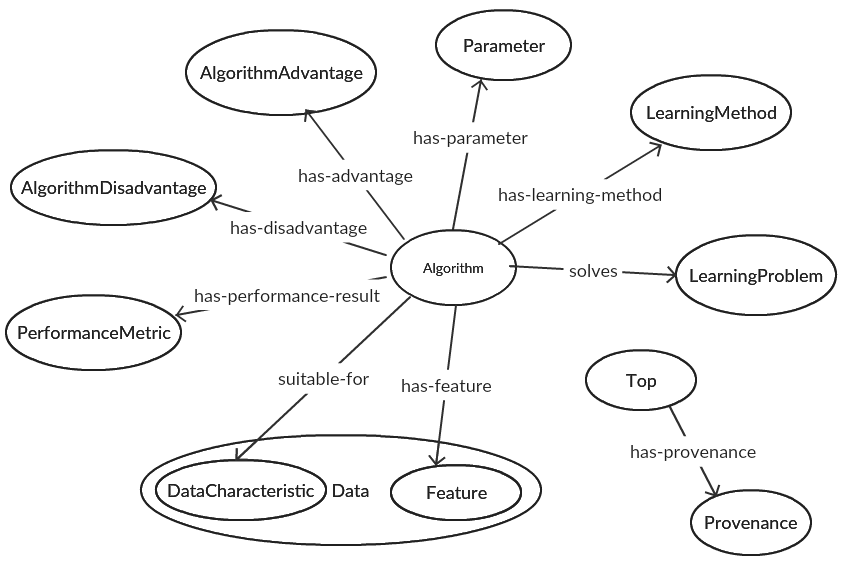
\includegraphics[width = 1 \linewidth]{img/ontologie_black.png}
        \caption{Vedere de ansamblu asupra ontologiei pentru machine learning: conceptul {\it Algorithm} 'si rolurile sale c'atre alte concepte.}
    \label{fig:onto}
\end{figure}

O vedere schematic'a asupra ontologiei apare 'in ~\ref{fig:onto}. 'In aceasta se pot observa rolurile care leag'a conceptul ML {\it Algorithm} de celelalte concepte din ontologie. Sunt expuse doar conceptele din primul nivel, excep'tie f'ac\i and clasa {\it Data} care este prezentat'a 'impreun'a cu cele dou'a subclase ale sale: {\it DataCharacteristic} 'si {\it Feature}. Imaginea eviden'tiaz'a datele con'tinute de ontologie: algoritmi, parametrii acestora, metode de 'inv'a'tare, problema de 'inv'a'tare pe care o rezolv'a, metrici de performan't'a, caracteristicile datelor 'si features, avantaje 'si dezavantaje, c\i at 'si informa'tii despre provenien'ta acestora.

\begin{figure}[h!]
    \centering
    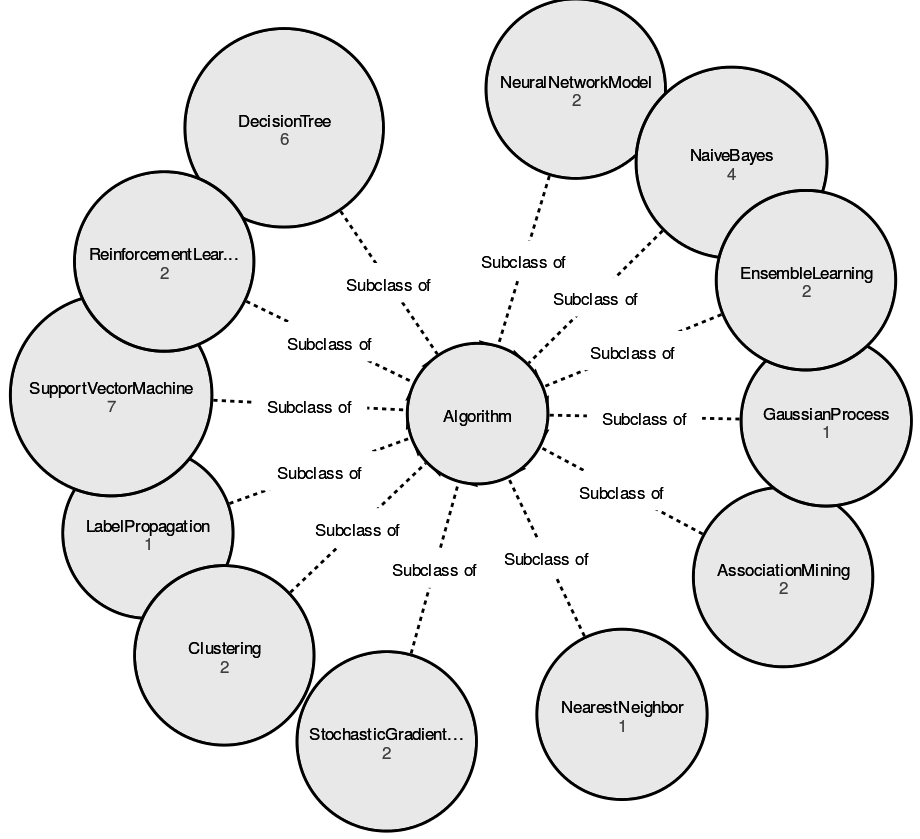
\includegraphics[width = 0.8 \linewidth]{img/algorithm_subclasses.png}
        \caption{Clasa {\it Algorithm}: diferiti algoritmi pentru ML}
    \label{fig:alg_sucls}
\end{figure}

Conceptul {\it Algorithm} este divizat 'in mai multe subconcepte care reprezint'a familii diferite de algoritmi, ce pot fi v'azute 'in Fig.~\ref{fig:alg_sucls}. Aduce 'impreun'a algoritmi care au metode de 'inv'a'tare supervizat'a, nesupervizat'a (cum ar fi clustering sau asociere), semi-supervizat'a 'si reinforcement. Cuprinde diferite varia'tii de algoritmi care sunt structura'ti 'in sublcase 'in func'tie de familia din care apar'tin: $DecisionTree$, $NeuralNetworkModel$, $NaiveBayes$, $SupportVectorMachine$, $LabelPropagation$ etc.

Similar conceptului de {\it Algorithm}, 'si parametrii sunt grupa'ti 'in clasa {\it Parameter} 'in func'tie de algoritmii c'arora le sunt asocia'ti. Figurile ~\ref{fig:subc_1} si ~\ref{fig:subc_2} ilustreaz'a acest fapt. Am ales divizarea parametrilor mai 'int\ia i 'in func'tie de familia de care apar'tin. Dac'a algoritmii din aceea'si familie nu folosesc aceia'si parametrii, am 'imp'ar'tit mai departe ace'sti parametrii 'in func'tie de indivizii c'arora le sunt asocia'ti. Parametrii compu'si apar'tin fiecare clasei c'areia 'ii descrie. 

\begin{figure}
    \centering
    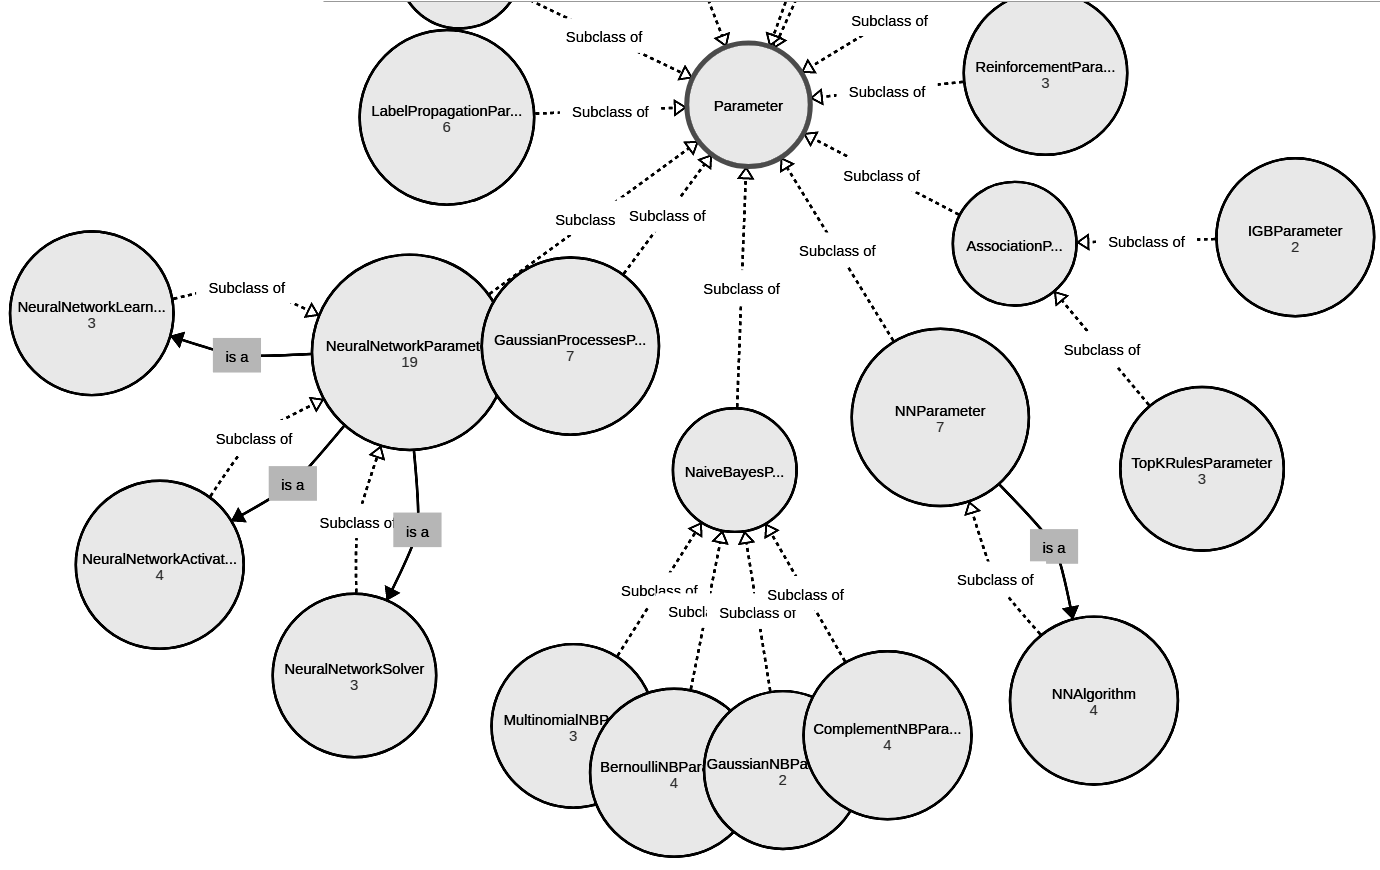
\includegraphics[width = 0.95 \linewidth]{img/properties_subcls_1.png}
        \caption{Prima parte a subconceptelor clasei $Parameter$}
    \label{fig:subc_1}
\end{figure}

\begin{figure}
    \centering
    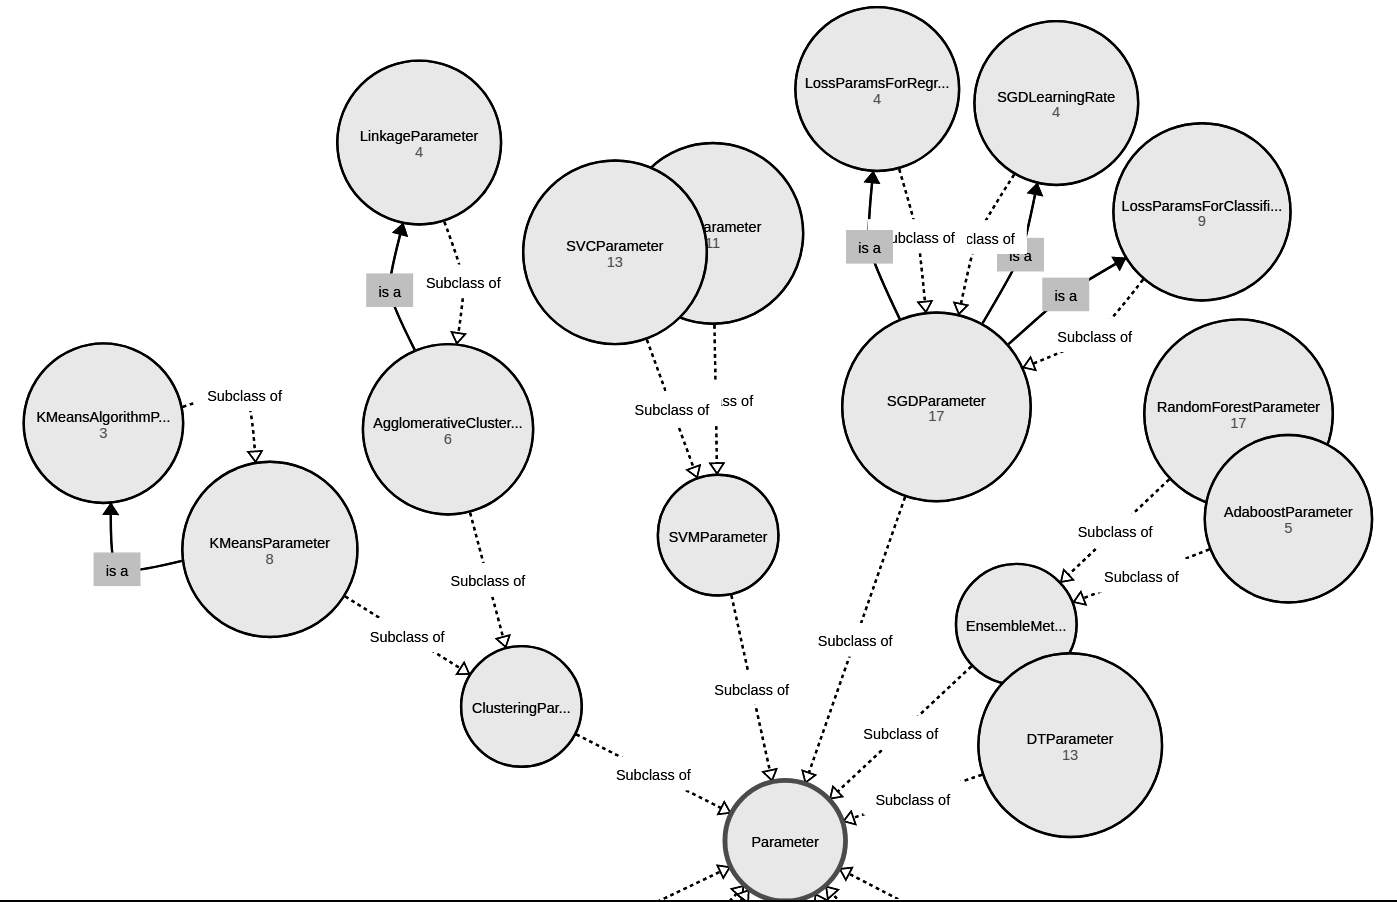
\includegraphics[width = 0.95 \linewidth]{img/properties_subcls_2.png}
        \caption{A doua parte a subconceptelor clasei $Parameter$}
    \label{fig:subc_2}
\end{figure}

Pentru popularea ontologiei ne-am bazat pe diferite tool-uri disponibile pentru ML. Pentru algoritmi pentru clustering, 'inv'a'tare semi-supervizat'a 'si superviza'ta, sursa principal'a de informa'tie este SciKit\footnote{https://scikit-learn.org/stable/}. Pentru association mining, am utilizat spmf\footnote{http://www.philippe-fournier-viger.com/spmf}. Datele despre reinforcement provin de la UNSW Sydney\footnote{https://www.cse.unsw.edu.au/~cs9417ml/RL1/algorithms.html}. 
%Being implemented taking into account good practices, our machine learning ontology can be further extended.


Ontologia a fost populat'a utiliz\ia nd Protege, acesta fiind o unealt'a automat'a pentru construirea ontologiilor. Permite ad'augarea conceptelor, a propriet'a'tilor 'si a indivizilor 'si genereaz'a un fi'sier 'in formatul dorit, OWL. Prezent'am in continuare exemple de implementare.

Proprietatea $has-learning-method$ prezint'a domeniul $Algorithm$ 'si codomeniul (range) $LearningMethod$ 'si este definit'a astfel:
\begin{lstlisting}[basicstyle=\footnotesize]

<owl:ObjectProperty rdf:about="http://www.semanticweb.org/machine-learning-ontology
                                #has-learning-method">
    <rdfs:domain rdf:resource="http://www.semanticweb.org/machine-learning-ontology
                                #Algorithm"/>
    <rdfs:range rdf:resource="http://www.semanticweb.org/machine-learning-ontology
                                #LearningMethod"/>
</owl:ObjectProperty>
\end{lstlisting}


 Clasa $Algorithm$ este definit'a astfel 'in fi'sierul OWL:
\begin{lstlisting}[basicstyle=\footnotesize]
    <owl:Class rdf:about="http://www.semanticweb.org/machine-learning-ontology
                        #Algorithm"/>
 \end{lstlisting}   

O subclas'a a clasei $Algorithm$, $EnsembleMethod$, con'tine 'in defini'tia sa o leg'atur'a c'atre superclas'a si un comentariu:
\begin{lstlisting}[basicstyle=\footnotesize]
    <owl:Class rdf:about="http://www.semanticweb.org/machine-learning-ontology
                        #EnsembleLearning">
        <rdfs:subClassOf rdf:resource="http://www.semanticweb.org
                             /machine-learning-ontology #Algorithm"/>
        <rdfs:comment>
            The goal of ensemble methods is to combine the predictions
            of several base estimators built with a given learning algorithm in
            order to improve generalizability / robustness over a single estimator.
        </rdfs:comment>
    </owl:Class>
    
\end{lstlisting}
Individul $classification$ face parte din clasa $LearningProblem$ 'si este definit astfel: 

\begin{lstlisting}[basicstyle=\footnotesize]
    <owl:NamedIndividual rdf:about="http://www.semanticweb.org
                        /machine-learning-ontology#classification">
        <rdf:type rdf:resource="http://www.semanticweb.org
                        /machine-learning-ontology#LearningProblem"/>
    </owl:NamedIndividual>
    
\end{lstlisting}


'In tabelul ~\ref{table:individuals_table} prezent'am pentru un exemplu de algoritm, $decisionTreeClassifier$, propriet'a'tile 'si indivizii din codomeniul acestora. 

\begin{table}[ht]
\caption{Indivizi ai ontologiei}
\centering                          % tabel centrat 
\begin{tabular}{|c|c|c|c|}          % 4 coloane centrate 
\hline\hline                        % linie orizontala dubla
Proprietate& Indivizi & Clasa indivizilor \\ [0.5ex]   % inserare tabel
%heading
\hline                              % linie orizontal simpla
solves & classification & LearningProblem  \\               % corpul tabelului 
has-learning-method & supervised
& LearningMethod  \\[1ex]           % [1ex] adds vertical space
has-parameter &  \begin{tabular}{@{}c@{}} maxFeature, presort \\ max\_depth, class\_weight\end{tabular} & DTParameter \\[1ex]

suitable-for & nonLinearModels & DataCharacteristic \\[1ex]

has-feature-characteritic & complexInteractions & Feature \\[1ex]

has-advantage & whiteBox, handlesColinearity & AlgorithmAdvantage\\[1ex] 
has-disadvantage & proneToOutliers, proneToOverfitting & AlgorithmDisadvantage \\[1ex]

has-provenance & scikitSupervised & Provenance \\[1ex]

\hline                              
\end{tabular}
  % titlul tabelului
\label{table:individuals_table}                % \label{table:nonlin} introduce eticheta folosita pentru referirea tabelului in text; referirea in text se va face cu \ref{table:nonlin}
\end{table}

'In acest tabel am inserat numai o parte din propriet'a'tile algoritmului $decisionTree$, acestea fiind multe la num'ar. 'In acest fel, am detaliat 'in ontologie o mare majoritate a algoritmilor insera'ti. 

%%%%%%%%%%%%%%%%%%%%%%%%%%%%%%%%%%%%%%%%%%%%%%%%%%%%%%%%%%%%%%%%%%%%%%%%%%%
\chapter{Testare 'si Validare}
\subsection{Scenariu de utilizare}
This section illustrates the capabilities of our system through a running scenario. 
Assume the user starts with the following question:

\begin{center}
{\it $Q_1$: Which are the instances of algorithms?}
\end{center}

This question can also be formulated as {\it"individuals of Algorithm"},
       {\it "print Algorithm instances"},
       {\it "show Algorithms individuals"},
        {\it"list Algorithm"} and it will be processed in the same way. 
The word "individual" can be replaced with "instance", but it may also be missing. Given that the plural of a concept can be a common usage, we also considered this case.
Based on the Quepy rule $R_1$ (formalised in section~\ref{sec:arch}) the corresponding SPARQL for $Q_1$ appears in Listing~\ref{lst:sparql:q1}:

%PREFIX owl:<http://www.w3.org/2002/07/owl#>
%PREFIX rdfs:<http://www.w3.org/2000/01/rdf-schema#>
\begin{figure}[h]
\begin{footnotesize}
\begin{lstlisting}[captionpos=b, caption=SPARQL formalisation for the query $Q_1$., label=lst:sparql:q1,
   basicstyle=\ttfamily,frame=single]
PREFIX rdf:<http://www.w3.org/1999/02/
           22-rdf-syntax-ns#>
PREFIX foaf:<http://xmlns.com/foaf/0.1/>
PREFIX skos:<http://www.w3.org/2004/02/skos/core#>
PREFIX quepy:<http://www.machinalis.com/quepy#>
PREFIX ml:<http://www.semanticweb.org/
           machine-learning-ontology#>

SELECT DISTINCT ?x0 WHERE {
  ?x0 rdf:type ml:Algorithm.
}
\end{lstlisting}
\end{footnotesize}
\end{figure}

Using Pellet, the answer $a_1$ is

\begin{center}
\begin{lstlisting}[basicstyle=\footnotesize]
{"head": { "vars": [ "x0" ]} ,
  "results": {
    "bindings": [
      {"x0":{"value":"gaussianProcessRegressor"}},
      {"x0":{"value":"oneClassSVM" }} 
      ...
      {"x0": {"value":"decisionTreeClassifier"}}]}}
\end{lstlisting}
\end{center}
where the variable $?x0$ stores the instances of the  {\it Algorithm} concept. 
The answer is obtained based on the following general inclusion axioms in description logic:

\vspace*{0.3cm}
\begin{tabular}{ll}
1. & $GaussianProcess  \sqsubseteq Algorithm$\\
2. & $SupportVectorMachine  \sqsubseteq Algorithm$\\
3. & $DecisionTree  \sqsubseteq Algorithm$\\
4. & $gaussianProcessRegressor: GaussianProcess$\\
5. & $oneClassSVM: SupportVectorMachine$\\
6. & $decisionTreeClassifier: DecisionTree$\\
\end{tabular}
\vspace*{0.3cm}

Pellet deduces from the axioms (1) and (2) that $GaussianProcess$, $DecisionTree$ and $SupportVectorMachine$ are subconcepts of $Algorithm$. Given axioms (4), (5) and (6), Pellet infers that $gaussianProcessRegressor$, $oneCLassSVM$ and $decisionTreeClassifier$ are also individuals in the concept $Algorithm$. 

Differently, using RDFLib, the answer is an empty list because RDFLib can't perform reasoning on given facts and it can't deduce that $gaussianProcessRegressor$, $oneCLassSVM$ and $decisionTreeClassifier$ are  individuals of $Algorithm$. 
In this case, if we wanted $DecisionTree$'s instances then RDFLib would have responded correctly with a list of individuals. 
For example, given the query in Listing~\ref{lst:sparql:dt} in which we ask for individuals of the $DecisionTree$ concept:


\begin{figure}[h]
\begin{footnotesize}
\begin{lstlisting}[captionpos=b, caption=SPARQL query for obtaining the instances of the DecisionTree concept., label=lst:sparql:dt,
   basicstyle=\ttfamily,frame=single]
SELECT DISTINCT ?x0 WHERE {
  ?x0 rdf:type ml:DecisionTree.}
\end{lstlisting}
\end{footnotesize}
\end{figure}

The answer $a_2$ computed by RDFLib is:

\begin{center}
\begin{lstlisting}[basicstyle=\footnotesize]
    [{ "x0": "decisionTreeRegressor"}, 
    ...
    {"x0": "decisionTreeClassifier"}, 
    {"x0": "id3"}]
\end{lstlisting}
\end{center}
\subsection{Performan't'a}

Am evaluat aplica'tia utiliz\ia nd un set de 10 'intreb'ari pe care le-am rulat de 100 de ori. Am calculat media ob'tinerii unei interog'ari SPARQL 'si um'arul de constr'angeri pe care 'il are aceasta, num'arul de indivizi din r'aspunsul dat de Pellet 'si timpul afl'arii acestui r'aspuns, num'arul de instan'te con'tinute de r'aspunsul dat de RDFLib 'si timpul 'in care acesta a fost ob'tinut. 

Am utilizat urm'atoarele 'intreb'ari, unde $TQ$ refer'a o 'intrebare de test (test question):
\newline

\begin{small}
\begin{tabular}{ll}
$TQ_1$ & list Algorithm individuals\\
$TQ_2$ & list DecisionTree individuals\\
$TQ_3$ & sarsa learning methods\\
$TQ_4$ & What are the advantages of kMeans?\\
$TQ_5$ & show details of identity\\
$TQ_6$ & Data subclass\\
$TQ_7$ & class of mlpRegressor\\
$TQ_8$ & algorithm that solves classification problem and has\\
 & supervised learning method and has feature \\
 & complexInteractions \\
$TQ_9$ & algorithms that do not have supervised learning  \\
& method \\
$TQ_{10}$ & algorithm suitable for nonLinearModels \\
& or shortDocuments\\
\end{tabular}
\end{small}

'In tabelul ~\ref{table:performance} pot fi observate rezultatele acestei analize. Datorit'a arhitecturii sistemului, timpul ob'tinerii r'aspunsurilor de la modulul $Translator$ este 'int\ia rziat cu aproximativ 1 secunda. 'In schimb, libr'aria Pellet extrage r'aspunsul 'intr-un timp foarte bun. De'si acesta a fost scopul acestei analize, nu am puut constanta o leg'atur'a clar'a 'intre num'arul de r'aspunsuri 'si timpul necesar execu'tiei 'intreb'arilor.
\begin{table}
\caption{Performan'ta sistemului}
\centering                          % tabel centrat 
\begin{tabular}{|c|c|c|c|c|c|c|}          % 4 coloane centrate 
\hline\hline                        % linie orizontala dubla
TQ &  Constr\ia ngeri  & Quepy  & Nr. de rezultate & Pellet  & Nr. de rezultate  & RDFLib \\ [0.5ex]   % inserare tabel
& SPARQL & time(ms) & Pellet & Time(ms) & RDFLib & time(ms)\\ [0.5ex]
%heading
\hline                              % linie orizontal simpla
$TQ_1$ & 1 & 1930 & 32 & 7  & 0 & 1902 \\[1ex]
$TQ_2$ & 1 & 1719 & 6  & 5 & 6 & 1691 \\[1ex]
$TQ_3$ & 3 & 1852 & 1  & 5 & 0 & 1782 \\[1ex]
$TQ_4$ & 3 & 1828 & 3  & 5 & 0 & 1899 \\[1ex]
$TQ_5$ & 3 & 1715 & 1  & 4 & 1 & 1657 \\[1ex]
$TQ_6$ & 2 & 1867 & 4  & 6 & 2 & 1672 \\[1ex]
$TQ_7$ & 2 & 1723 & 3  & 6 & 2 & 1667 \\[1ex]
$TQ_8$ & 8 & 1915 & 1  & 11 & 0 & 1786 \\[1ex]
$TQ_9$ & 3 & 1830 & 13  & 4 & 0 & 1774 \\[1ex]
$TQ_10$ & 6 & 2057 & 4 & 8 & 0 & 2083 \\[1ex]

\hline                              
\end{tabular}
  % titlul tabelului
\label{table:performance}                % \label{table:nonlin} introduce eticheta folosita pentru referirea tabelului in text; referirea in text se va face cu \ref{table:nonlin}
\end{table}

% 'In urma unei analize mai profunde 'si separate a $Translatorului$ am ob'tinut rezultatele din tabelul ~\ref{table:performance_tr}. 
% \begin{table}
% \caption{Performan'ta modulului $Translator$}
% \centering                          % tabel centrat 
% \begin{tabular}{|c|c|c|c|c|c|c|}          % 4 coloane centrate 
% \hline\hline                        % linie orizontala dubla
% TQ &  Constr\ia ngeri  & Quepy  & Nr. de rezultate  & RDFLib \\ [0.5ex]   % inserare tabel
% & SPARQL & time(ms)  & RDFLib & time(ms)\\ [0.5ex]
% %heading
% \hline                              % linie orizontal simpla
% $TQ_1$ & 1 & 23  & 0 & 23 \\[1ex]
% $TQ_2$ & 1 & 3 & 6 & 8 \\[1ex]
% $TQ_3$ & 3 & 2 & 0 & 19 \\[1ex]
% $TQ_4$ & 3 & 1  & 0 & 19 \\[1ex]
% $TQ_5$ & 3 & 3  & 1 & 19 \\[1ex]
% $TQ_6$ & 2 & 3  & 2 & 17 \\[1ex]
% $TQ_7$ & 2 & 3  & 2 & 17 \\[1ex]
% $TQ_8$ & 8 & 5  & 0 & 41 \\[1ex]
% $TQ_9$ & 3 & 4  & 0 & 24 \\[1ex]
% $TQ_10$ & 6 & 2 & 0 & 32 \\[1ex]

% \hline                              
% \end{tabular}
%   % titlul tabelului
% \label{table:performance_tr}                % \label{table:nonlin} introduce eticheta folosita pentru referirea tabelului in text; referirea in text se va face cu \ref{table:nonlin}
% \end{table}


% Acestea de confirm'a faptul c'a transmisia datelor dintre $Translator$ 'si $Reasoning\ Service$ dureaz'a mult, dar ne arat'a 'sii o leg'atur'a 'intre numarul de rezultate ob'tinute de RDFLib 'si timpul de execu'tie pentru ob'tinerea acestora. Se poate observa c'a timpul scade odat'a cu cre'sterea num'arului de rezultate.
%%%%%%%%%%%%%%%%%%%%%%%%%%%%%%%%%%%%%%%%%%%%%%%%%%%%%%%%%%%%%%%%%%%%%%%%%%%
\chapter{Manual de Instalare 'si Utilizare}

\section{Instalarea sistemului}
\section{Manual de utilizare}



%%%%%%%%%%%%%%%%%%%%%%%%%%%%%%%%%%%%%%%%%%%%%%%%%%%%%%%%%%%%%%%%%%%%%%%%%%
\chapter{Concluzii}

\section{Contribu'tii 'si realiz'ari}
\section{Dezvolt'ari ulterioare}


%\addcontentsline {toc}{chapter}{Bibliography} 
\bibliographystyle{IEEEtran} 
\bibliography{thesis}%same file name as for .bib

\appendix
\chapter{Sec'tiuni relevante din cod}

\begin{verbatim}
 /** Maps are easy to use in Scala. */
object Maps {
  val colors = Map("red" -> 0xFF0000,
                   "turquoise" -> 0x00FFFF,
                   "black" -> 0x000000,
                   "orange" -> 0xFF8040,
                   "brown" -> 0x804000)
  def main(args: Array[String]) {
    for (name <- args) println(
      colors.get(name) match {
        case Some(code) =>
          name + " has code: " + code
        case None =>
          "Unknown color: " + name
      }
    )
  }
}
\end{verbatim}

\chapter{Alte informa'tii relevante (demonstra'tii etc.)}

\textcolor{green}{LISTA DE INTREBARI PERMISE}

\chapter{Lucr'ari publicate (dac'a exist'a)}

Agentul explicabil pentru 'inv'a'tare automat'a descris 'in aceast'a lucrare a fost prezentat 'si 'in articolul "Towards Explainable Machine Learning Using  Natural Language Processing and Ontologies". Articolul este trimis la "IEEE 15th International Conference on
Intelligent Computer Communication and Processing (ICCP 2019)" 'si se afl'a in curs de verificare. Cu o variant'a restr\ia ns'a a acestuia am participat la "Conferin'ta 'Stiin'tific'a a Studen'tilor Sec'tiilor de Calculatoare 2019".
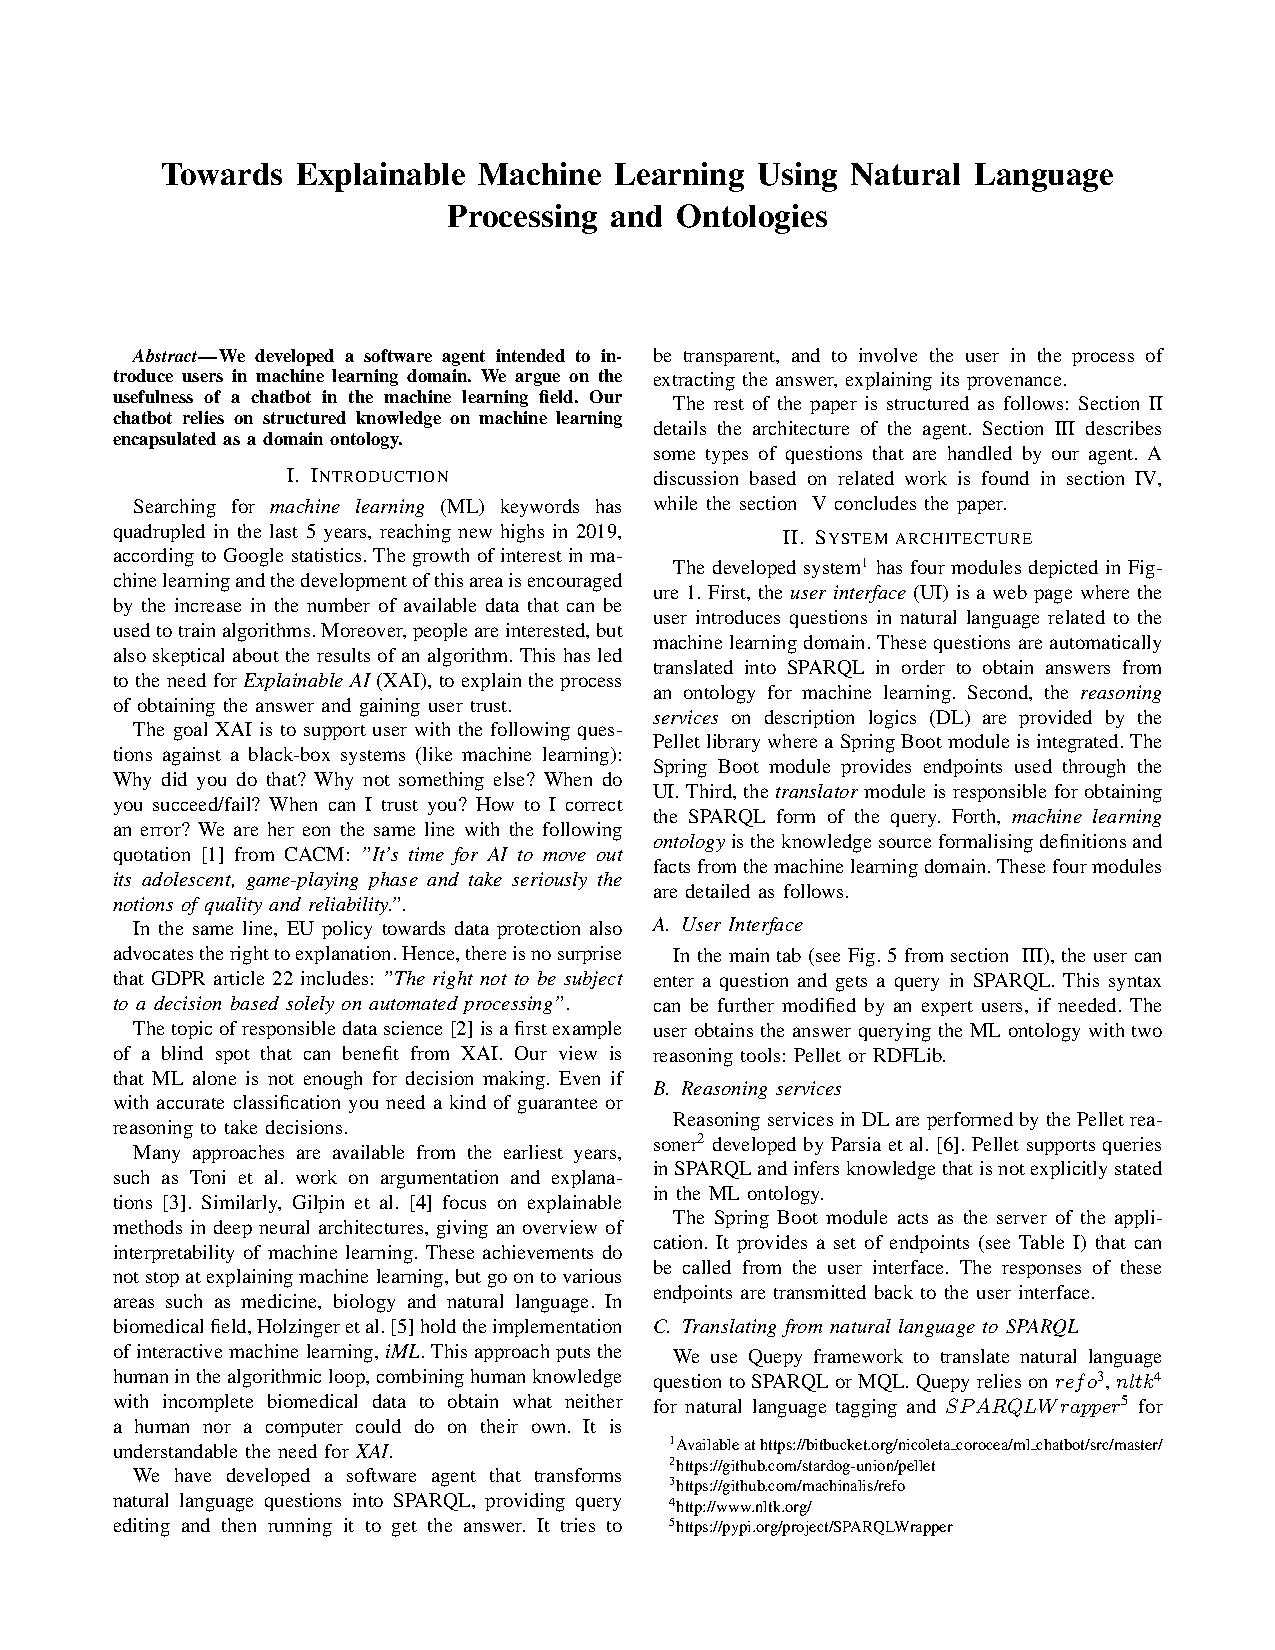
\includepdf[pages=-,pagecommand={},width=\textwidth]{articol_extins.pdf}


\end{document}
